The system is used primarily identify certain patterns in different types of multivariate time-series. In this section, we highlight several examples - the first from synthetically generated data followed by two real world datasets. Finally we describe some other examples of the use of system.  These datasets can be found on the StreamStory system (\url{http://streamstory.ijs.si}). 

\subsection{Prediction Evaluation}

This first experiment is intended to test the validity of our model. The model was constructed on simulated data of 
an electric motor and is shown in Figure \ref{fig:example-motor}. 
\begin{figure*}[]
  	\centering
  	\begin{subfigure}[b]{.48\textwidth}
	  	\centering
	  	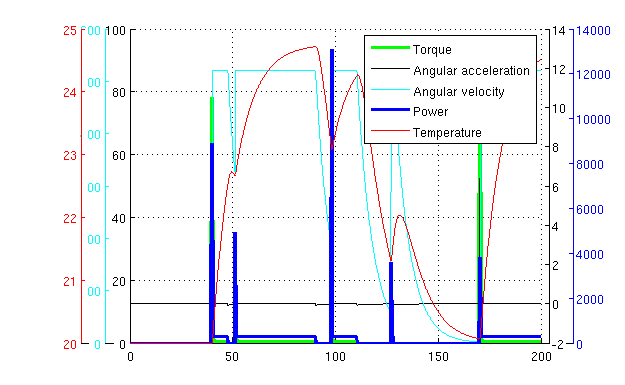
\includegraphics[width=\columnwidth]{simulation-processed}
  		\caption{\label{fig:simulation-chart}}
	\end{subfigure}
  	\begin{subfigure}[b]{.48\textwidth}
	  	\centering
	  	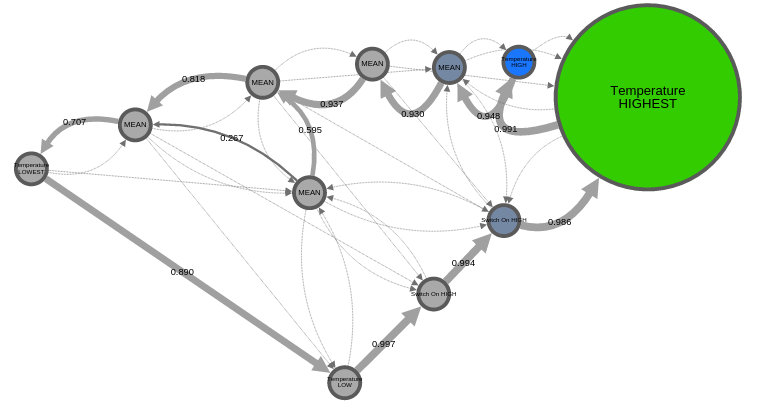
\includegraphics[width=\columnwidth]{model-motor-simulated}
  		\caption{\label{fig:simulation-model}}
	\end{subfigure}
  	\caption{Simulation of an electric motor plotted as a standard time-chart \ref{fig:simulation-chart} and our qualitative model \ref{fig:simulation-model}.}
  	\label{fig:example-motor}
\end{figure*}
The simulation starts in the leftmost state of Figure~\ref{fig:simulation-model} with the motor in a stationary state
and the power switch turned off. Then \lstopar{an invisible user} randomly, sampled from an exponential distribution,
toggles the ``on" switch. Once the switch is on, as the rotation increases, the model starts moving in the counter clockwise
direction towards the large green state on the right. This state represents the \lstopar{equilibrium} when the temperature
gained through friction equals the temperature lost to the ambient and the \lstopar{signals} become \lstopar{stationary}.
Once the power switch is toggled again, the rotation slowly halts due to friction and the process goes from right to
left in the counter clockwise direction.

To conduct the experiment we generated two dataset: a training set and a test set. Both datasets
contained $200k$ observations. We built a StreamStory model with 20 lowest-level states on the training set using two attributes:
angular velocity and temperature. The training dataset was then replayed through the model and the finest scale states were stored. We then used
the stored states to calculate the transition probabilities and compared them to the models' jump chain $\Pi$. Since a lot of these probabilities were zero, we decided to use only the probabilities that
are non-zero either in the jump chain or in the probabilities calculated from the history. We then
computed the mean absolute error of the non-zero probabilities which resulted in $MAE=0.05$ or $5\%$.

In another experiment we tested the models predictive power. Two StreamStory models were built: (a) one 
model using the same attributes as in the first experiment, while in the second model (b), we used
the logical switch signal to model state transitions. The models were trained on the same dataset
as in the first experiment. Before the process jumped, we extracted the next state probabilities
and used the state with the highest probability as the predicted next state. We then computed
the prediction accuracy as the ratio between the number of correct predictions and the total number
of jumps (total number of predictions). In this experiment model (a) scored $0.845$ while model
(b) scored $0.904$.

\lstopar{
The experiment was conducted by simulating the characteristic curve (linear characteristics) of a typical direct current permanent magnet electric motor \cite{book:1107411}.
}

\subsection{Weather Data}
\label{sec:experiments-weather}

The example below shows our model generated on monthly rainfall and temperature data
collected over the course of 20 years between 1920 and 1940 in Nottingham, England.

\begin{figure}[h!]
	\centering
	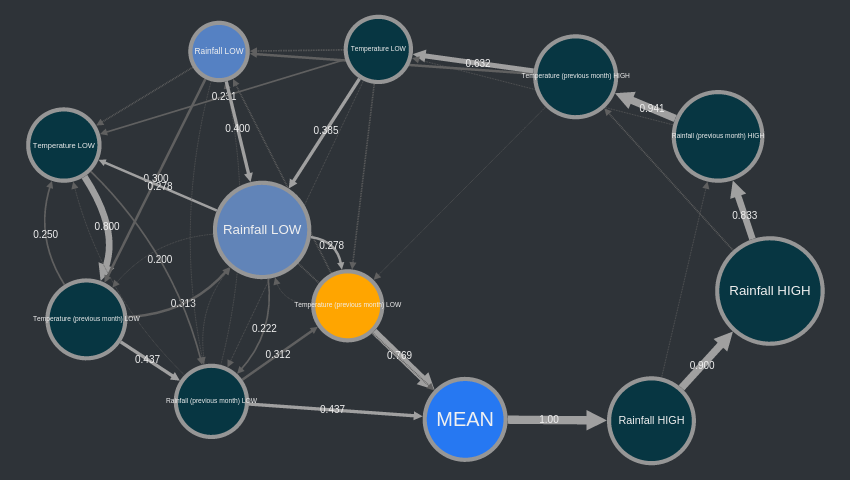
\includegraphics[width=\columnwidth]{example-weather}
	\caption{Qualitative representation of temperature and rainfall data collected over the course of 20 years. The yearly timeline flows in the clockwise direction with the right-most state representing the summer, the bottom states representing autumn, the left-most states representing winter and the top states representing spring.}
	\label{fig:example-weather}
\end{figure}

The model was generated using the raw rainfall and temperature data, lifted into a four dimensional space.
\lstopar{Lifting was done as suggested in Section \ref{sec:preliminaries} by appending the previous sample to the current sample, effectively adding two new dimensions}.

The states on the right hand side represent the 
summer states, while the states on the left represent winter states. The yearly timeline flows in the clockwise direction with the spring states residing on the bottom of the figure and the autumn
states on the top.

Interestingly, in this dataset, the rainfall and temperature are very correlated and the auto labeling feature
choose high rainfall as the most significant feature of the summer states. This correlation can be seen
from the attribute histogram shown in Figure \ref{fig:histograms-summer}.

Using our model, we can clearly see how the summer and winter dynamics differ. While the summer states seem to be quite deterministic, with a high probability of jumping into the next state in the clockwise direction, the transition probabilities in the winter states are much more uniform, suggesting larger fluctuations in the weather during the winter.

\begin{figure}[h!]
	\centering
	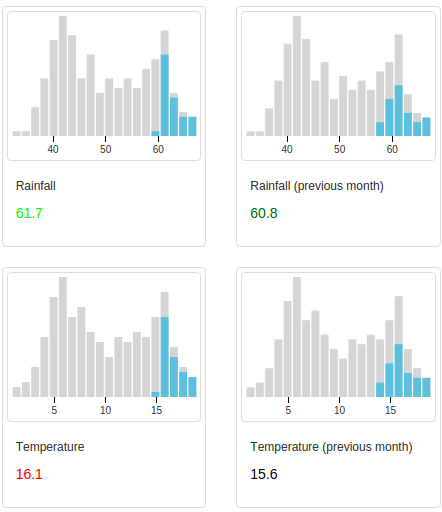
\includegraphics[width=0.7\columnwidth]{histograms-summer}
	\caption{Histograms of the signals in one of the summer states in the weather data shown in Figure \ref{fig:example-weather}. The histograms suggest a high correlation between the temperature and rainfall in the dataset.}
	\label{fig:histograms-summer}
\end{figure}

\subsection{GPS Data}

The second example was created using raw GPS coordinates collected using a smartphone between years 2012 and 2015.
The data represents the everyday movement of a European computer science researcher. Figure \ref{fig:example-geo}
shows our qualitative representation of this data on a high level with 8 states.

\begin{figure}[h!]
	\centering
	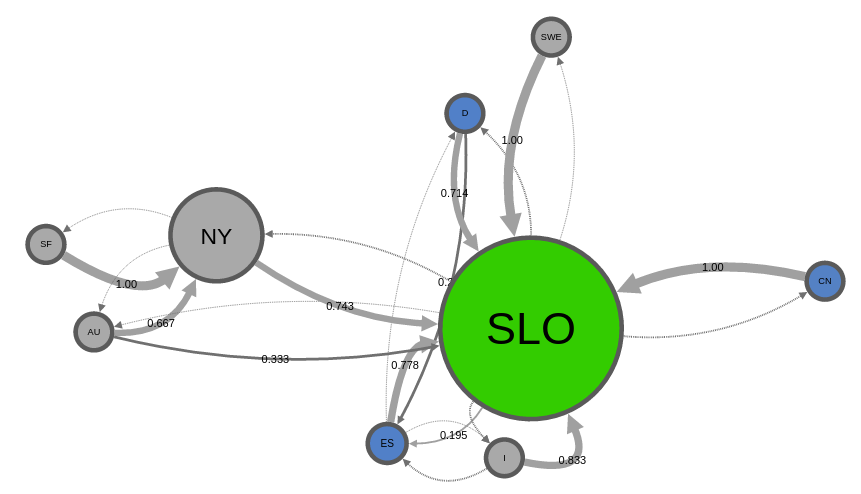
\includegraphics[width=\columnwidth]{geo-states}
	\caption{Qualitative representation of GPS data representing the movements of a European researcher, collected over the course of four years. Using our system, we were able to identify the most typical locations where the person traveled, including the USA, Germany, Italy, Spain, Sweden, China and Slovenia, their associated states are shown labeled using appropriate country/city codes.}
	\label{fig:example-geo}
\end{figure}

From the figure, we can see that the system was able to identify the most typical locations of this persons
movements.

They spent most of the time in the large green state representing Slovenia. On the European continent, the system was able to identify Germany, Sweden and Spain where the person frequently attends meetings as well as Italy, which represents a transition state \lstopar{airport}. The small state on the right is China, where they went for vacation in 2015. The states on the left represent the USA with the largest of the three representing New York city the person spent the 2014 summer and the smaller two states representing San Francisco and Austin, Texas.

\subsection{Traffic Data}

Our final example, shown in Figure \ref{fig:example-traffic-multiscale}, shows a multi-scale representation of two traffic counters positioned on a highway ring around Ljubljana, Slovenia. In this example, the data is the number of cars per hour passing each counter, sampled every $15$ minutes. \lstopar{In this example, we lifted the dataset, as suggested in Section \ref{sec:preliminaries}, into a four dimensional space by appending reading from three hours in the past to the current signal.} 

\begin{figure}[h!]
  	\centering
  	\begin{subfigure}[b]{.48\columnwidth}
	  	\centering
	  	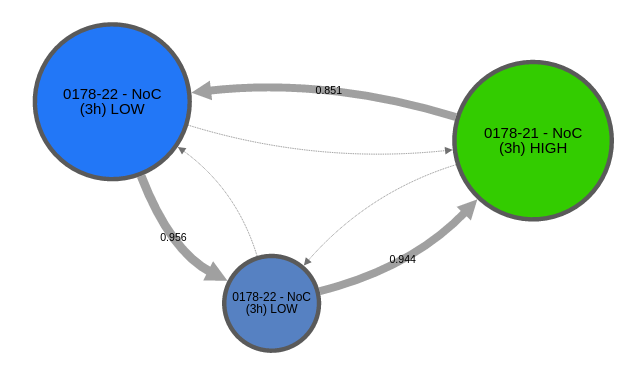
\includegraphics[width=\columnwidth]{traffic-coarcest}
  		\caption{\label{fig:traffic-coarcest}}
	\end{subfigure}
  	\begin{subfigure}[b]{.48\columnwidth}
	  	\centering
	  	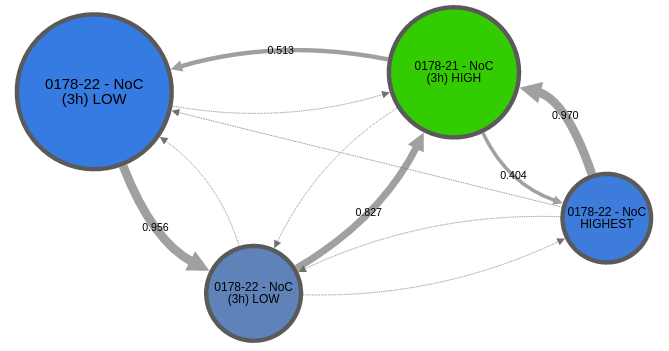
\includegraphics[width=\columnwidth]{traffic-coarcer}
  		\caption{\label{fig:traffic-coarcer}}
	\end{subfigure}
	\begin{subfigure}[b]{.48\columnwidth}
	  	\centering
	  	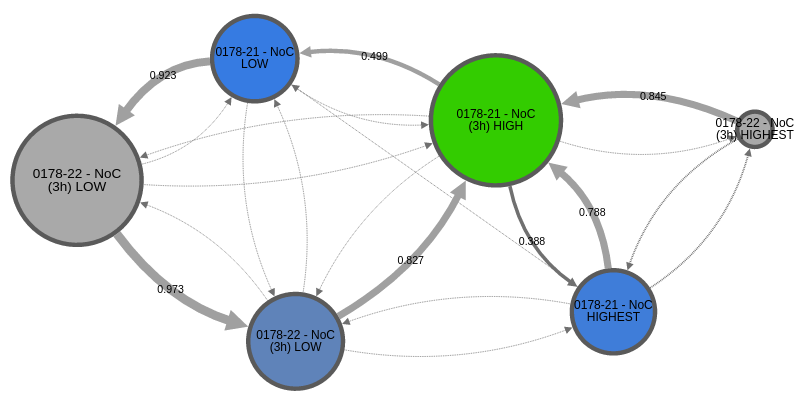
\includegraphics[width=\columnwidth]{traffic-middle}
  		\caption{\label{fig:traffic-middle}}
	\end{subfigure}
	\begin{subfigure}[b]{.48\columnwidth}
	  	\centering
	  	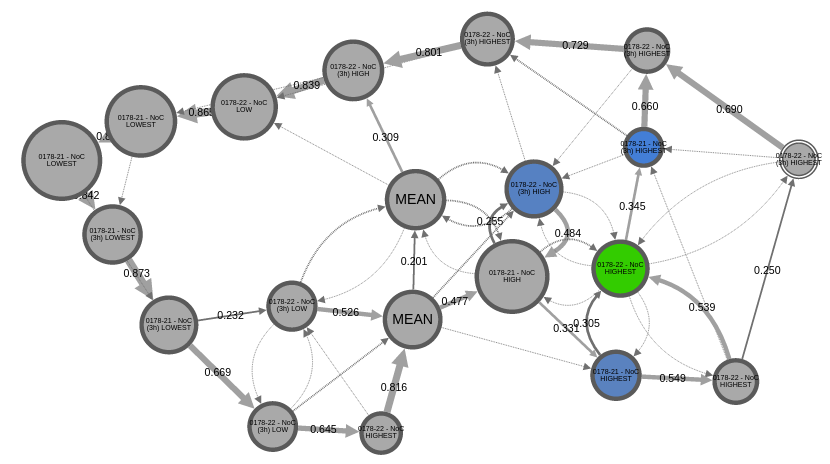
\includegraphics[width=\columnwidth]{traffic-finest}
  		\caption{\label{fig:traffic-finest}}
	\end{subfigure}
  	\caption{A multi-scale representation of two traffic counters positioned on Ljubljana's highway ring from a coarse scale \ref{fig:traffic-coarcest} down to the finest scale \ref{fig:traffic-finest}. From our model we identified what we believe is the typical daily cycle on the ring flowing in the counter clockwise direction. On the finest scale in Figure \ref{fig:traffic-finest} one can clearly distinguish the nightly and daily dynamics with the nightly dynamics being very deterministic while there is a low of noise in the daily dynamics brought by various events.}
  	\label{fig:example-traffic-multiscale}
\end{figure}

On a coerce scale, with only three states, we were able to identify the typical daily cycle on the ring. The cycle starts with the leftmost state in Figure \ref{fig:traffic-coarcest} representing the night state with a low number of cars detected by both sensors lasting from approximately $9$PM to $6$AM. It then moves in the counter clockwise direction into the bottom state representing the morning. The morning state has a relatively high number of cars detected on both sensors, lasting from $7$ to approximately $9$AM. The state on the right of Figure \ref{fig:traffic-coarcest} represents the day state lasting from $10$AM to approximately $9$PM.

When zooming into a finer scale, shown in Figure \ref{fig:traffic-coarcer}, the rightmost state gets split into two states. The top-left of the two new states (green) now represents noon and evening and has a moderate number of cars with an average of $907$ and $631$ cars per hour for the two counters respectively. From this state, the system goes either back into the night state or into the afternoon state on the right of Figure \ref{fig:traffic-coarcer} with the highest number of cars detected on both sensors, with an average of $1240$ and $1290$ cars per hour. This state lasts from approximately $3$PM to $6$PM when the system jumps back into the moderate day state.

When zooming even further into Figure \ref{fig:traffic-middle}, an interesting thing happens. The system detects a small state which typically occurs on Friday evening and is shown on the right of Figure \ref{fig:traffic-middle}. This is a time when most of the student leave the town and go home for the weekend and when people leave for weekend vacations.
Finally when zooming in even further into Figure \ref{fig:traffic-finest} a new structure appears. Each state now represents a smaller time interval with the nightly states in the top left of the figure and the daily states on the bottom right. It is not surprising that the transitions in the nightly states seem a lot more deterministic than in the daily states. Indeed, at night not a lot of cars drive on the ring while during the day various events introduce noise into the system.

\primoz{
\begin{itemize}
\item Here we also need some examples of where its not useful -  a few different scales and we need references on the data. These can be deliverables. 
\item Also we should show how much information we lose over different scales.
\end{itemize}}

\subsection{Domain Experts}
In the above examples, the discovered states could be interpreted by non-experts. We have also tested the system in more specialized settings. One example the system was tested on measurements from an oil drilling platform\footnote{Unfortunately, at the time of submission, we were not cleared to share the results of the analysis, including an evaluation on useability.}. In this data, natural recurrent behaviour was detected.  The model also detected an ``event,'' where certain equipment failed and drilling needed to be halted.  

%A second example is based on a manufacturing plant. In this case, we cannot 

